\documentclass[letterpaper,11pt,oneside,final]{uicthesis}
\usepackage{amsfonts, amsmath, amsthm, amssymb, epsfig, graphicx, float}
\usepackage[longnamesfirst,square,sort&compress, comma]{natbib}
\usepackage[xindy,style=index]{glossaries}
\usepackage{bera}
\usepackage[utf8]{inputenc}
\usepackage{lipsum}
\usepackage{xcolor}
\usepackage[color]{soul}

% Configuration
	% Thesis title
	\newcommand{\thesisTitle}{Temporal Analysis of Wire Transfers for Fraud Detection}
	% Thesis author
	\newcommand{\thesisAuthor}{Luca Cioria}
	% Author's previous degrees
	\newcommand{\authorDegrees}{M.Sc., Politecnico di Milano, Apr 2014}
	% Current degree (Thesis's degree)
	\newcommand{\thesisDegree}{Master of Science in Computer Science}

\usepackage[unicode,
			pdftex,
			plainpages=false,
			linktoc=all,
			hyperindex,
			breaklinks=true,
			citecolor=green,
			urlcolor=blue
		   ]{hyperref}
\hypersetup{
	pdftitle={\thesisTitle},
	pdfauthor={\thesisAuthor}
}

% Style
% !TEX root =  ../thesis.tex

\def\chapterautorefname{Chapter}
\def\sectionautorefname{Section}
\def\subsectionautorefname{Section}
\def\subsubsectionautorefname{Section}
\def\figureautorefname{Figure}
\def\tableautorefname{Table}

% Double spacing for text
\linespread{2} % 2
% No square brackets in bibliography
\makeatletter
\renewcommand\@biblabel[1]{#1.}
\makeatother
% Bibliography style
\renewcommand\bibname{}
\renewcommand{\bibsection}{\section*{}}
% Single spacing list of abbreviations
\renewcommand*{\glsgroupskip}{}
% Hyperref fix
\def\texorpdf #1#2{\texorpdfstring{#1{#2}}{#2}}


% Acronyms (to appear in the List of Abbreviations)
\makeglossaries
% !TEX root =  ../thesis.tex

\newacronym{UI}{UI}{User Interface}
\newacronym{GUI}{GUI}{Graphical User Interface}


\begin{document}

	\begin{titlepage}
	\topskip0pt
	\vspace*{\fill}
	\begin{spacing}{1.5}
	\begin{center}

		{\Large \thesisTitle}

		\vspace{4.2cm}
    BY\\

    LUCA CIORIA\\
		\vspace{0.2cm}
    Laurea Magistrale, Politecnico di Milano, Milan, Italy, 2014

		\vspace{3.2cm}
    THESIS\\
		\vspace{0.2cm}
    Submitted as partial fulfillment of the requirements\\
    for the degree of Master of Science in Computer Science\\
    in the Graduate College of the\\
    University of Illinois at Chicago, 2015
		\vspace{0.5cm}
    \begin{flushleft}
    Chair: Venkat\\
    Committee:  Lenore Zuck, Stefano Zanero
    \end{flushleft}

	\end{center}

	\end{spacing}
	\vspace*{\fill}
	\end{titlepage}

	\dedication
		 % !TEX root =  ../thesis.tex
\setcounter{page}{2}

\begin{flushright}
	\emph{To anyone I ever learnt from.}
  \vspace{1cm}
  % \emph{To my family and friends, \\ who supported me all these years} \\
\end{flushright}


	%\acknowledgements
		%% !TEX root =  ../thesis.tex





	\setcounter{tocdepth}{2}
	\tableofcontents
	\listoftables
	\listoffigures
	% Remember to run makeglossaries thesis
		% \glsaddall
		% \printglossary[title=LIST OF ABBREVIATIONS]

   \summary \label{summary}
   This thesis aims to improve the current systems to identify fraudolent bank tansactions. We start by analyzing the state of the art, in particular the work done in the BankSealer project, focusing on the temporal analysis of user profiles. We then suggest a new approach at identifying anomalous shifts in user spending patters, that should prove more general and effective than the current one.

   After having defined a possible new system, we test its effectiveness and generality with a fully working prototype implementation against a set of over a million real bank transactions, and conclude by explaining the main success areas of the new approach, and the possible areas of improvement for future work.

	\chapter{Introduction} \label{introduction}
		% !TEX root =  ../thesis.tex

\section{Motivations}

This work is born from the need to improve some specific areas of anomaly detection in bank transfers, in particular what we will call here `temporal profile analysis', as it was already called in the BankSealer framework. As we will see in later chapter, our model of a temporal profile is very different from what was done in BankSealer, but is intended to provide a superset of functionalities, being more general, and therefore we kept the name.

In particular, in BankSealer the temporal profile is able to analyze a very limited set of features, built ad hoc for it. These features are:
\begin{description}
  \item[total amount] total amount spent in a month
  \item[number of transactions] total number of transactions performed in a month
  \item[maximum daily number of transactions] maximum number of transactions performed in a single day in the last month
\end{description}

These three features are not defined in a generic way, but rather concieved to fit well in a temporal analysis of the user. They have two main issues: first, they're not comprehensive with respect to all the possible features to analize. Second, they only consider grand totals, and not how these totals split up in categories. We will delve further in these issues and our approach to solve them in the next section.

\section{Towards a solution}

To better understand the issue of grand totals, consider this example.

A user averages at 100 transactions per month, mostly around a few hundreds euros each. In the current month, we see 120 transactions, which is not a big enough increase to go over our threshold. However, if we analyzed how these transactions distributed over their amount, we'd see that we have 30 transactions of just 10 euros each. Considering not only the grand total, but how transactions distribute within a profile, we can notice a shift and alert that the current month has a high anomaly level regarding the amount.

This approach may seem very similar to what is done in BankSealer's local profile, but it differs in a few crucial ways and can therefore complement the local profile. In the local profile a transaction was tested against a user local profile for a specific feature to derive a level of anomaly. In our temporal profile, a whole profile is tested with an average of recent profiles, to detect a shift in the overall behavior of the user. Following the previous example, the local profile would probably have raised suspicion over some (possibly all) the 10 euros transactions in questions if the anomaly derived from the amount had been sufficient. However, the fact that they were 30 transactions wouldn't in any way have been taken into account for the current month, while this information is a signal that those transactions could be frauds. Also, if the transactions varied for other features, such as time of the day, it's very possible that only some of them would show up in the local profile as anomalous, and the analyst wouldn't realize that there were actually 30 transaction around 10 euros.

With our approach, we identify the problem at a higher level: the whole profile, not the single transaction. Then, we try to bring it back to transactions by selecting those transactions that were mostly responsible for the shift in behavior. This can be used as a complement to the local profile in various ways: either integrating its signal in an overall anomaly value, or showing anomalous proiles separately and letting the analyst drill down in the details for each transaction thanks to the local profile anomaly value.

	\chapter{State of the Art} \label{soa}
		% !TEX root =  ../thesis.tex

\section{Related work}

This thesis is born to address limitations in the BankSealer fraud detection framework, and therefore the majority of the citations and reference to related work will be for BankSealer~\cite{banksealer}.

More in general, various works have addressed similar issues in the past but the focus has mostly been towards Credit Card frauds instead of bank transfers. Also, the limited availability of real data from banks, mainly due to privacy concerns, has slowed research in the field.

\section{BankSealer}

BankSealer is a semi-supervised analysis tool for bank frauds. It is developed to work as a support for decisions made by analysts, and therefore it works with a ranking based system, computing an anomaly score for each transactions. Also, the anomaly score is transparent, in the sense that its value can be decomposed and understood by a human.

It works by creating profiles that represent the spending habits of clients, and then comparing new transactions to these profile in order to assess how much they deviate from such profiles. In particular, it uses three types of profiles for each user: local, temporal and global profiles. The local profile is the most important one as it is used to compute an anomaly level for each transaction. The temporal profile tries to find anomalies at a higher level (e.g.: total number of transactions in a month) and the global profile computes the anomaly of the user as a whole with respect to all the other users.

The system proved to be effective in ranking fraudolent transactions as top priority, in particular thanks to the local profile analysis. Further improvements are necessary on the temporal profile analysis (the objective of this work) and the global profile analysis, which had positive effects on undertrained users but did not result very effective in raising the performance of the analysis on trained users.

	\chapter{User Profiles and Distance Measure} \label{profiles}
		% !TEX root =  ../thesis.tex

Before being able to understand how profiles change in time and find anomalous profiles and transactions, we need to understand how a profile is defined and computed.

After preliminary definitions and an explanation of the different types of profiles, we will focus more on their mathematical representation (the histogram) and its properties, with the objective of defining a distance function able to satisfy our requirements.

\section{Definition of User Profile}

In order to define a User Profile, we will first introduce a few preliminary definitions.

\begin{description}
  \item[user] a single client of the bank, be it a private or a company, identified by a unique code in the dataset.
  \item[feature] a dimension of a transaction, which can be of type Integer, Real or Categorical
  \item[window] a period of time on which transactions are grouped and a profile is defined. For each window, only one profile exists, and vice versa. Windows in this thesis will in general be of one month.
  \item[bin selection] the procedure of mapping a value to a bin in a histogram
\end{description}

A profile is computed from a set of transactions that belong to the same time window, and it is composed of a set of histograms, one for each feature. The sum of each histogram is equal to the total number of transactions. Each histogram is composed of 2 or more bins, where the value of each bin is defined as the number of transactions for which the value of the feature related to the histogram is included in the set of bin values.

\subsection{Histograms and their properties}

Now we shift the focus from the overall user profile to the properties of a single histogram. A single histogram represent a pattern in the user transactions over that feature. For instance, let us take the feature `amount' in consideration. The amount is simply the monetary value of a transaction, expressed in euros. A histogram mostly flat, such as in figure \ref{fig:flat_histogram}, means that the user makes transactions of all amounts indiscriminately. If the histogram is mostly skewed to the left, the user will prefer smaller transactions; if to the right, bigger transactions.

\begin{figure}[h]
\centering
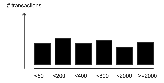
\includegraphics[width=250]{images/flat_histogram.pdf}
\caption{Histogram representing the distribution of transactions over the `amount' feature}
\label{fig:flat_histogram}
\end{figure}

To understand this, only the shape of the histogram is relevant, and can therefore be normalized to have sum one and interpreted as a discrete probability distribution.

We refer to a histogram with the notation $H$, and to the value of bin $i$ with $H(i)$.

We follow the classification of histograms as proposed in \cite{histogram}, which divides histograms in three families based on their type of measurement:

\begin{description}
\item[ordinal] the values are ordered, such as numbers or more in general anything that can be ordered.
\item[nominal] the values are a finite set of possible categories, without any ordering implied.
\item[modulo] the values are ordered in a `ring' where the rightmost values are close to the leftmost ones, as in the arithmetic modulo operation.
\end{description}

\section{Distance between histograms}

In order to compute how profiles change over time, we need to introduce the concept of a distance between histograms. This topic is central to this thesis, and will be explored in depth, as it provides the basis for the whole temporal profile analysis system.

We refer to the distance between histograms $H(A)$ and $H(B)$ as $d(H(A), H(B))$.
The distance function will need to be specified over histograms of the same family, and possibly be specialized for each one.

To fulfill the requirements of the temporal analysis, the distance function will have to satisfy a few properties. To better understand why these properties are necessary, an understanding of the system design is useful and can be found in chapter~\ref{design}.

In the following list we will explain which properties it will have to satisfy and why such properties are necessary.
\begin{description}
  \item[reflexive] $d(H(A), H(A)) = 0$. Since with our distance function we will be measuring the variations in spending profiles over time, we have to assign a null variation to a profile that does not change at all.
  \item[commutative] $d(H(A), H(B)) = d(H(B), H(A))$. The necessity for this property is less obvious, because we might want to consider shifts in certain directions as more relevant than in others. However, our design treats all variations in the same way, without giving a meaning to the direction of such variations. For instance, if a user changes her spending profile from mostly low amount transactions to mostly high amount transactions, we want to produce the same distance value as if the shift was reversed. This ensures that our approach remains generic.
  \item[non negative] $d(H(A), H(B)) \geq 0$. Considering that we require our function to be reflexive, and therefore have a $0$ point, having a negative function would mean differentiating distances in 2 directions, such as increase and decrease. As explained in the previous paragraph, we do not want to assign a meaning to the direction of the shift, but only to its magnitude, therefore the function should be non negative.
  \item[positional] for ordinal and modulo histograms, the distance between bins should be taken into account. In other words, the distance function should be a function of the order of the bins, in additions to being a function of their values. Of course, not any relation between the order of the bins and the final distance value is acceptable. Our goal is to reduce the distance when bins with a value $\geq 0$ are close together, since small variations in positions should be considered noise. This property will be discussed in greater details in the following paragraphs.
\end{description}

Before continuing to an analysis of possible distance functions, a quick note on a property that we did not require: \textbf{triangle inequality}. This property says that, for any three histograms $A$, $B$ and $C$, $d(H(A), H(B)) \leq d(H(A), H(C)) + d(H(C), H(B))$.

An example of distance function that does not satisfy this property is the euclidean distance to the power of 2, defined as the sum over each dimension $i$ of $(H(A,i) - H(B,i))^2$. In this case, longer distances will be accounted for in a more than linear fashion. This is not in contrast with our design, as hypothetically it might be possible that such a function resulted in higher performance, accounting more for greater shifts than smaller ones.

Based on a few tests using the euclidean function to the power of $x$, with $x > 1$, we did not find any big difference (positive or negative). In conclusion, we do not require this property and leave experimenting with distance functions that violate it as a possible future work.

\subsection{Positionality: noise and information}

In this section we will delve further in what we mean by positionality and why we think this is essential for our work.
First, let us make an example to better understand:\\
$H(A) = [1, 0, 0, 0, 0]$\\
$H(B) = [0, 1, 0, 0, 0]$\\
$H(C) = [0, 0, 0, 0, 1]$

The desired behavior of our distance function will depend on the type of these histograms:
\begin{description}
  \item[nominal] all distances should be equal
  \item[ordinal] $d(H(A), H(B)) < d(H(A), H(C))$ since the bins containing a 1 are further apart in the second case
  \item[modulo] $d(H(A), H(B)) = d(H(A), H(C))$ since the bins containing a 1 are next to each other, if we see the histogram as a ring
\end{description}

We say that the distance is \textit{shuffling invariant} for nominal histograms and \textit{shuffling dependent} for ordinal and modulo histograms.

We think this property is desirable in our scenario, where a shift in spending habits from transactions around 500 euros to transactions around 800 euros is less relevant than a shift to transactions around 5000 euros.

The issue of positionality can be interpreted in terms of information and noise. Continuing with the amount example, a shift in the order of 100 euros can be interpreted as noise, while a greater shift in the order of thousands of euros conveys real information. We can then formulate our goal in a more high level version: we want our distance function to \underline{consider relevant information and be resilient to noise in the histogram variations}.

We will now review a few distance functions that can be applied to histograms and finally select the one that better satisfies all the properties we need.

\subsection{Vector representation based distances}

Histograms can be seen as vectors and any distance function that work with vectors can therefore be used. The two easiest distances are:
\begin{description}
  \item[city block] sum over each dimension $i$ of $|H(A,i) - H(B,i)|$
  \item[euclidean] squared sum over each dimension $i$ of $(H(A,i) - H(B,i))^2$
\end{description}

As with all vector based distances, these distances are shuffling invariant and therefore do not satisfy positionality at all. We still included them here because, when complemented with appropriate filtering, they can serve our purpose, as explained in the following paragraphs.

\subsection{Minimum distance of pair assignments}

The MDPA (minimum distance of pair assignments) is a distance function that, at a basic level, satisfies all the properties we require, as shown in \cite{histogram}. To define the MDPA consider two sets of n elements, A and B, which define histograms $H(A)$ and $H(B)$. The MDPA is intuitively equal to the minimum total cost of the `moves' that we need to make in order to transform the first histogram in the second one. A move is defined as subtracting $x$ from bin $i$ and adding it to bin $j$. The cost of a move is $x * d(i, j)$ where $d(i, j)$ is the linear distance between the two bins.

This distance can be used for ordinal and modulo histograms as it takes into account the position of bins. Moreover, efficient algorithms exist for computing the MDPA distance. We have implemented the algorithm for the ordinal type and tested it, as documented in section \ref{sec:mdpa_test}, in order to see if it fit our requirements.

The problem is that in these algorithms the distance $d(i, j)$ between bins is considered to be a linear distance. We think that this is not optimal in our scenario, since the meaning of such distance depends on the feature measured by the profile associated with the histogram and other distances could be necessary. In particular super-linear distance functions could make more sense in real world situations, where for instance $d(i, j), i=0, j=4$ should be more than double than $d(i, j), i=0, j=2$.

To verify this assumption, we tested the MDPA function and compared it to our approach (as explained in the next section) and found a substantial improvement with the latter. Of course, defining a custom distance $d(i, j)$ that is non linear is possible in MDPA, but leads to a generic optimization problem with exponential complexity. Efficiency being a key component of our design, we discarded this direction of research.

\section{Low-pass filtered euclidean distance}

Our approach is based on a completely different technique: instead of finding another distance algorithm that takes bin position into account, we apply a low-pass filter to the histograms and then apply a normal euclidean distance.

In this way we can achieve our goal of reducing noise and taking into account the overall shape of the histogram, which represents the spending pattern of the user, rather than the small variations in each bin. 

The low-pass filter we decided to use is the gaussian filter, which is a very well known filter used to remove high frequency noise, reducing the variance in the values of the histogram.

The two dimensional gaussian smoothing filter, also known as gaussian blur, is often used in computer vision to perform contour and shape detection. In our situation, it solves a similar problem in revealing the shape of the histogram.

\subsection{Gaussian function and Weierstrass transform}

The gaussian function with mean $\mu = 0$ is defined as:
\begin{displaymath}
  \frac{1}{\sigma\sqrt{2\pi}}e^{-\frac{x^2}{2\sigma^2}}
\end{displaymath}

The smoothing filter that results from the convolution of the input histogram with the Gaussian function is the Weierstrass transform.

Using the weierstrass transform, each bin in the smoothed histogram is the weighted average of its surrounding bins, using the gaussian function to compute the weights.

For instance, the weight assigned in the weighted average to a bin next to the one being computed is given by the gaussian function where $x = 1$, being $x$ the distance between the bins. We can consider as insignificant bins with distance $x > 3\sigma$.

This method can account for different types of histograms and can be tuned by adjusting the parameter $\sigma$ of the gaussian function in order to specify how much the histograms should be smoothed before computing their euclidean distance.

In particular, we have as always three types of histograms to account for:

\begin{description}
  \item[nominal] no smoothing should be applied, the euclidean distance can be computed directly
  \item[ordinal] smoothing should be applied, if the weighed average would includes bins outside of the histogram range (for instance, when computing the average for the first or last bin) it should be limited to those available.
  \item[modulo] smoothing should be applied, but in this case when bins are outside of the histogram range they will be taken from the other end of the histogram, following the rules of the arithmetic modulo operator.
\end{description}

\subsection{Preservation of properties}

The euclidean function is reflexive, non-negative and commutative but not positional. We need to prove that, applying the gaussian filter to both input histograms before applying the euclidean distance, we are preserving those properties and in addition satisfying positionality.

\begin{description}
  \item[reflexive] Since the gaussian blur is a deterministic mathematical transform that will always give the same result given the same input, we can state that \\
    $d(F(H(A)), F(H(A))) = 0$.
  \item[commutative] Following the same logic, the transform does not affect commutativity of the euclidean distance.
  \item[non-negative]
    However transformed, the input of the euclidean distance does not affect its non negativity (the difference over each dimension is squared).
  \item[positional] First, the euclidean distance can be rewritten like this:
    $$\sqrt{\sum_{n=0}^{n} (a_i-b_i)^2} = \sqrt{\sum_{n=0}^{n} a_i^2+b_i^2-2a_ib_i} = \sqrt{\sum_{n=0}^{n} a_i^2 + \sum_{n=0}^{n} b_i^2 - \sum_{n=0}^{n} 2a_ib_i}$$
    The first and second sum are independent of the order of bins, while the third one multiplies bins in the same position. Therefore, the higher the overlap of the two histograms, the lower their distance. The gaussian filter will transform the histograms decreasing their variance. The higher the $\sigma$ value, the lower the variance. Consider a normalized histogram $H(A)$ of length $n$ (whose integral is 1):
      $$\lim_{\sigma\to\infty} a_i = \frac{1}{n}, 0 \leq i < n $$
      Therefore, after a gaussian filter, bins will be closer to the average value of $\frac{1}{n}$ and overlap will have increase, reducing their distance. Since the total area can be conserved simply by normalizing the histogram after the filter, the first two sums are not affected.
      Now, to explain why this satisfy the requirements of positionality, we can see that the gaussian filter will transform each bin only based on at most $\ceil{3\sigma}$ bins on each side. Therefore, if bins are far apart, the overlap will not increase for low enough $\sigma$ values. The closer they are, the more the overlap will increase and the final distance decrease. This is exactly what positionality requires, as defined before and for the goal of our work.
\end{description}

\subsection{Example of the low-pass filter euclidean distance}

Let us take two histograms, $H(A)$ and $H(B)$ defined as:
\begin{align}
  H(A) = [1,5,7,2,3,9,2]\\
  H(B) = [0,3,6,2,1,2,1]
\end{align}

The first step to compute the distance is to process these histograms with a gaussian smoothing filter, as previously explained. To understand the effects of such filtering, look at figure \ref{fig:sigma_difference}. The original histogram, printed in black, is $H(A)$. In green we can see the smoothed version of the histogram, on the left with $\sigma = 0.5$ and on the right with $\sigma = 1$. As you can see, raising the value of the $\sigma$ parameter increases the smoothing effect.

\begin{figure}[h]
\centering
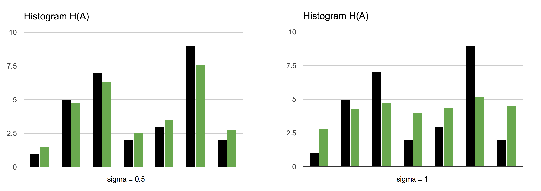
\includegraphics[width=450]{images/sigma_difference.pdf}
\caption{In green the smoothed version of the histogram in black, for two different values of the $\sigma$ parameter}
\label{fig:sigma_difference}
\end{figure}

In figure \ref{fig:smoothed_a_b} we can see the two histograms along with their smoothed version at $\sigma = 0.5$. The final distance will be the euclidean distance between the smoothed version. These are the distances at different smoothing levels:
\begin{align}
  \sigma = 0.5, \text{distance} = 6.91\nonumber\\
  \sigma = 1, \text{distance} = 6.09\nonumber\\
  \sigma = 2, \text{distance} = 5.53\nonumber
\end{align}
Without smoothing the distance would have been $7.74$, higher than any of the other distances. This is because, thanks to smoothing, we can take into account the fact the similarity of values in close bins. For instance, take $H(A,1) = 1$ which became $H(A,1) = 0.4$ after smoothing, thanks to the presence of the bin next to it which had a value of $3$.

\begin{figure}[h]
\centering
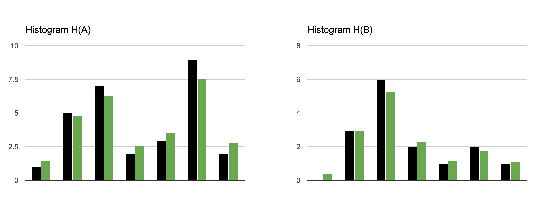
\includegraphics[width=450]{images/smoothed_a_b.pdf}
\caption{Original and smoothed versions of the two histograms $H(A)$ and $H(B)$ at $\sigma = 0.5$}
\label{fig:smoothed_a_b}
\end{figure}


	\chapter{System Design} \label{design}
		% !TEX root =  ../thesis.tex

In this chapter we will talk about the overall design of the temporal profile analysis system. This system is based on the definition of user profiles for each time window, and then the analysis of how these profiles evolve in time.

\section{Overall system design}

The system, at a very high level, is composed of four main parts, as illustrated in figure~\ref{fig:system_design}.

First, transactions are grouped by time windows and user profiles are generated. One user profile is produced for each combination of user, time window and feature. For instance a profile could be associated with:\\ \texttt{user: 941825, time window: january 2015, feature: spent amount}.

Then, the distance from the past profiles is computed for each profile. The past is an average of the last few profiles for that user and feature, in the preceding time windows. This average is weighed on exponentially discounted weights the further in the past we go.

The third step is to analyze these distances and select anomalous ones, those that are greater than a dynamic threshold based on the standard deviation of past distances.

Lastly, after having identifies the profiles with anomalous distances, we select the transactions in these profiles that are the best candidates as to being responsible for the anomaly in the distances.

The final goal is to present these findings in a structured way to an expert analyst, detailing where each figure came from in the analysis, so that the analyst better know where to look and what to give more importance too also based on their experience.

\begin{figure}[h]
\centering
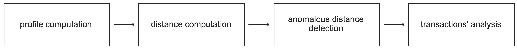
\includegraphics[width=450]{images/overall_system_design.pdf}
\caption{Overall system design of the temporal profile analysis system}
\label{fig:system_design}
\end{figure}

\section{Profiles and distances computation}

After a time window has passed (e.g.: the first of the month), the following procedure that creates the user profiles for the last time window and computes its distance is executed for each user. This process is illustrated in figure \ref{fig:distance_computation}.

\begin{enumerate}
  \item for each feature, a \textbf{profile} is built by creating the histogram representing the distribution of the values for that feature over all transactions in the last window. In figure \ref{fig:distance_computation} we build the profile for the amount feature. The amount is defined as a real number and divided into buckets based on its values and an interval defined for each bin.
  \item the exponentially discounted average of the past profiles is computed, defined as the average of the value of each bin in the last $N$ profiles, with weights exponentially discounted the more we go further in to the past. All histograms have the same number of bins, and so does the average histogram.
  \item the distance between the current profile and the \textbf{average} profile is computed, following the distance rules associated with this feature. In the example of the amount, we have an ordinal histogram, therefore we use our definition of distance that applies a smoothing filter and an euclidean distance. If we were analyzing the feature \texttt{hour of the day}, which generates a modulo histogram, we would have used the modulo distance (where the smoothing filter is circular). Lastly, for nominal features such as \texttt{type} we would have used directly the euclidean distance.
\end{enumerate}

\begin{figure}[h]
\centering
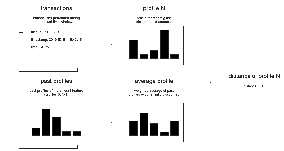
\includegraphics[width=450]{images/distance_computation.pdf}
\caption{Overall system design of the temporal profile analysis system}
\label{fig:distance_computation}
\end{figure}

\section{Anomalous distance detection}

At this stage we have, for a combination of user and feature, a chronological series of profiles (one for each time window). For each profile, we know its distance from the past, how much that profile changed compared to the past ones. This represents a shift in spending habits of the user, who maybe began working at night or spending larger sums, or whose transactions might in fact be frauds.

The current step identifies the profiles whose distance is greater than normal. How do we define the threshold for normality? The standard deviation of the $M$ previous distances, where $M$ is a tunable parameter, is computed. The threshold is dynamically defined for each profile as this standard deviation times a sensitivity parameter $\alpha$. In this way, we can mark as anomalous only those profile that move apart from the current mean by more than $\alpha$ times the typical standard deviation.

The following procedure summarizes what we have just explained, and is illustrated in figure \ref{fig:distance_analysis}:

\begin{enumerate}
  \item the \textbf{standard deviation} of the $M$ previous distances is computed, where $M$ is a parameter to be chosen
  \item the \textbf{anomaly} of the current profile is computed as:
    \begin{displaymath}
      \frac{\text{distance}-\text{average distance}}{\text{std dev of previous distances}}
    \end{displaymath}
  \item profiles with an anomaly level greater than a \textbf{threshold} $\alpha$ to be chosen are notified to the analyst
\end{enumerate}

\begin{figure}[h]
\centering
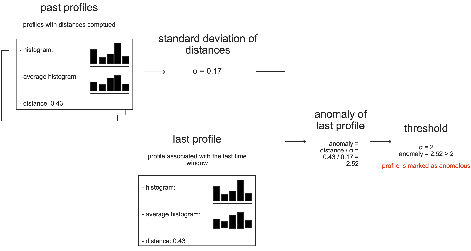
\includegraphics[width=450]{images/distance_analysis.pdf}
\caption{Analysis of the distances between profiles to determine anomalous profiles}
\label{fig:distance_analysis}
\end{figure}

\section{Transactions' analysis}
\label{sec:transactions_analysis}

The last step of our system is to try to identifies those transactions part of the anomalous profiles that could be responsible for such anomaly. For example, if we have an anomalous profiles for the feature amount, we select those features that were the most atypical in terms of amount, in a similar way to what is done in the local profile in BankSealer \cite{banksealer}.

While this might seem redundant with respect to the local profile at first, what it does is very different. Transactions are not marked as anomalous because individually they differed from the typical user behaviors, but because they contribute to an overall behavioral shift. This is to be combined with the information we get form the local profile, so that fraudulent transactions that ordinarily would have passed by the local profile can be brought up by our temporal analysis.

To select the interesting transactions we have adopted a simple approach: search for bins which diverge the most from the average, and take those transactions as interesting. We stop when the distance, recomputed without considering these bins, falls under the anomaly threshold.

We will explain this in more detail in the next paragraphs, but first an important element to be considered is anomaly caused by absence rather than presence. Distance is symmetric, and the same anomaly level can be caused by an increment in transactions (for instance, with amount around 500 euros) and by a decrement of such transactions. It is however impossible to collect transactions that contributed to the anomaly if a decrement happened, and also less likely that the problem is associated with an attempted fraud.

The procedure (illustrated in figure \ref{fig:transactions_analysis}) is as follows:

\begin{enumerate}
  \item we sort the bins of the last histogram in decrescent order by the absolute difference of their values compared to the average histogram.
  \item we take the first bin. If its value is greater than the one in the average histogram, we select as interesting all the transactions in the bin. If it's lower, we mark the bin as anomalous because of absence.
  \item we recompute the distance without considering the previous bin (practically, we do this setting it to the same value as the corresponding bin in the average histogram). If the distance is still above the threshold of anomaly, we start over at step 1, otherwise we have finished collecting interesting transactions.
\end{enumerate}

\begin{figure}[h]
\centering
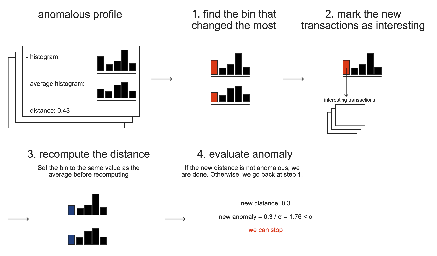
\includegraphics[width=450]{images/transactions_analysis.pdf}
\caption{Algorithm to find the most interesting transactions in an anomalous profile}
\label{fig:transactions_analysis}
\end{figure}

	\chapter{Implementation} \label{implementation}
		% !TEX root =  ../thesis.tex

A fully working prototype has been implemented to test the system design. The prototype has been run against real transactions provided by a bank institution, as will be explained in more details in the Test chapter. The prototype is written in ruby, an object oriented programming language that is well suited for fast prototyping and data manipulation. It is intended to run against a static dataset and not suited for online production data analysis, even though the main components are fully general and could be reused in an online implementation.

\section{Components of the prototype}

The prototype at a high level is a ruby program that runs against a MySQL database. The database is used both as data input, containing the raw transactions that were given by the bank institution, and as data output with profiles and analysis results.

In the next paragraphs we will provide a detailed description of the components of the prototype, following the processing order from the raw transactions to the final analysis.

\subsection{preprocessing}
Raw transactions from the bank are preprocessed to a normal form, where each record is composed by a set of defined features. The preprocessing step includes the removal of data not necessary for the analysis (e.g.: error messages on transactions), the definition of derived features (e.g.: the feature `hour of the day' is derived from the transaction's timestamp) and the simplification of features (e.g.: the `transaction type' is simplified from a complex set of domain specific types to a simpler distinction between `same bank transfers' and `SEPA transfers').

\subsection{Profile creation}
Transactions in normal form are grouped by user id. For each user, transactions are divided in groups based on the time window definition, in this prototype set to one month. Then, for each feature, a profile is created based on the feature configuration. The profile is then saved as a record in the database, identified by user, month and feature and containing its histogram representation.

\subsection{Average profile computation}
For each profile in the database, an average profile of the previous months (for the same user and feature) is computed. The average includes previous profiles with an exponential discount applied, based on profile configuration.

\subsection{Distance computation}
For each profile, the distance between the profile and the average profile associated with it is computed and stored. The distance is calculated based on the configuration of the distance function for that specific profile.

\subsection{Distance variance computation}
The standard deviation and mean of the previous distances is computed for each profile. A configurable amount of time windows is considered, and only if enough windows are available the result is saved, in order to avoid unreliable results.

\subsection{Anomaly computation}
An anomaly value is computed for each profile. The anomaly is defined as:
\begin{displaymath}
  \text{anomaly} = \frac{\max(0, d - \overline{d})}{\sigma}
\end{displaymath}
where $d = \text{distance}$, $\overline{d} = \text{average distance}$, $\sigma = \text{std dev of distances}$.

\subsection{Threshold}
The profiles with an anomaly value greater than the value of the threshold parameter for that feature are selected as anomalous. The threshold value is to be tuned experimentally for each feature, and in the prototype we have tested many different threshold values as explained in chapter \ref{test}.
While being important to select a good threshold value, this processing step is mainly intended to minimize false negative. In fact, one of the basic principles on which also banksealer operates is that we need to order transactions based on their probability of being frauds, being transparent on why they were selected, rather than just labeling them as frauds or not. In this scenario, the threshold parameter is useful in removing the majority of profiles for which we cannot reliably give an anomaly value, but then the selected profiles will be presented alongside their anomaly value, and ordered accordingly for the human analyst to process and evaluate.

\subsection{Transaction extraction}
As last step, from each selected profile a set of transactions is extracted following the rules outlined in \ref{sec:transactions_analysis}. Selected transactions are then saved to the database and form the starting point for the analyst operations. In a production environment, this information would be intergrated with the local profile analysis performed by banksealer, in which case the selected transactions could have their overall anomaly value raised in addition to being marked as anomalous by the temporal analysis.
We want to stress that our work is not a binary classifier, dividing transactions in fraudolent or not, and it is therefore important to associated the anomaly value of the profile with each selected transaction, so that it will be rendered in the correct order in the analyst interface.

	\chapter{Test} \label{test}
		% !TEX root =  ../thesis.tex


To test our temporal profile analysis system, we focused on a few scenarios where the typical local profile analysis would fall short and tried to see if the temporal analysis could help in identifying anomalous transactions. Our tests are based on a mixture of real data, taken from the transaction databased made available by our bank partner, and syntetic data. Syntetic data is used mainly to inject transactions that should be recognized as frauds, and in certain cases to create specific speding profiles to test.

\section{Detection of normal amount transactions}

This test is designed to spot anomalous behaviors in the number of transactions. We take a user that performs on average 30 transactions per month, with an amount linearly distributed between 0 and 5000 euros. We then inject 10 transactions in a specific month, having an amount of 50 euros. These transactions will not be considered suspicious by the local profile analysis because they fall in the range of normality with respect to their amount. Also, the previous temporal analysis system, as defined in banksealer~\cite{banksealer}, is not really able to detect the problem because it only analyzes the total number of transactions. The addition of 10 transactions in a month to a user that had, in the past, between 20 and 40 transactions per month, is not enough to trigger the old temporal profile system.

We ran the test on syntetic data, generating 100 users that would match this spending profile, and injecting in all of them anomalous transactions as explained above. The results of the test depend heavily on the sensitivity thresholds used. In table \ref{tab:conf_1_06} we see the confusion matrix resulting from a threshold $\alpha = 0.6$. The first thing to evaluate is the \textbf{recall}:
\begin{displaymath}
\text{recall} = \text{TP} / (\text{TP} + \text{FN}) = 66\%
\end{displaymath}
We refer to true positives as $\text{TP}$, false negatives as $\text{FN}$ and so on.
The recall, while not perfect, is in itself a good sign and can certainly be useful when combined with the other analysis methods. However, the precision of the system is, as expected, less than optimal:
\begin{displaymath}
\text{precision} = \text{TP} / (\text{TP} + \text{FP}) = 52\%
\end{displaymath}

\begin{table}[h]
\centering
\begin{tabular}{lllll}
\cline{1-2}
\multicolumn{1}{|c|}{\textbf{\begin{tabular}[c]{@{}c@{}}true positive\\ 66\end{tabular}}} & \multicolumn{1}{c|}{\textbf{\begin{tabular}[c]{@{}c@{}}false positive\\ 60\end{tabular}}} &  &  &  \\ \cline{1-2}
\multicolumn{1}{|c|}{\textbf{\begin{tabular}[c]{@{}c@{}}false negative\\ 34\end{tabular}}} & \multicolumn{1}{c|}{\textbf{\begin{tabular}[c]{@{}c@{}}true negative\\ 1040\end{tabular}}} &  &  &  \\ \cline{1-2}
 &  &  &  &  \\
 &  &  &  &
\end{tabular}
\caption{CONFUSION MATRIX $\alpha = 0.6$}
\label{tab:conf_1_06}
\end{table}

We will now see how changing the threshold affects these measures.

\subsection{How to choose a threshold value}

In the precedent paragraph we tested the accuracy and recall of our system with a threshold of $0.6$. This threshold has been chosen because it maximizes the \textbf{F1 score}, which is the harmonic mean of precision and recall:
\begin{displaymath}
F_1 = 2 \cdot \frac{\mathrm{precision} \cdot \mathrm{recall}}{\mathrm{precision} + \mathrm{recall}}
\end{displaymath}

This measure is a good indicator of a balance between precision and recall, which tries to be general, but is not optimal for our situation. In particular, we consider recall more important than precision, because we want in the end to signal almost all transactions that could be interesting, and we are prepared to lose some ground on the number of false positives, thus reducing precision.

In tables \ref{tab:conf_1_07} and \ref{tab:conf_1_05} we see how the numbers change with a shift of $+0.1, -0.1$ on our threshold parameter.


\begin{table}[h]
\centering
\begin{tabular}{lllll}
\cline{1-2}
\multicolumn{1}{|c|}{\textbf{\begin{tabular}[c]{@{}c@{}}true positive\\ 75\end{tabular}}} & \multicolumn{1}{c|}{\textbf{\begin{tabular}[c]{@{}c@{}}false positive\\ 92\end{tabular}}} &  &  &  \\ \cline{1-2}
\multicolumn{1}{|c|}{\textbf{\begin{tabular}[c]{@{}c@{}}false negative\\ 25\end{tabular}}} & \multicolumn{1}{c|}{\textbf{\begin{tabular}[c]{@{}c@{}}true negative\\ 1008\end{tabular}}} &  &  &  \\ \cline{1-2}
 &  &  &  &  \\
 &  &  &  &
\end{tabular}
\caption{CONFUSION MATRIX $\alpha = 0.5$. RECALL $75\%$, PRECISION $45\%$}
\label{tab:conf_1_05}
\end{table}

\begin{table}[h]
\centering
\begin{tabular}{lllll}
\cline{1-2}
\multicolumn{1}{|c|}{\textbf{\begin{tabular}[c]{@{}c@{}}true positive\\ 59\end{tabular}}} & \multicolumn{1}{c|}{\textbf{\begin{tabular}[c]{@{}c@{}}false positive\\ 49\end{tabular}}} &  &  &  \\ \cline{1-2}
\multicolumn{1}{|c|}{\textbf{\begin{tabular}[c]{@{}c@{}}false negative\\ 41\end{tabular}}} & \multicolumn{1}{c|}{\textbf{\begin{tabular}[c]{@{}c@{}}true negative\\ 1051\end{tabular}}} &  &  &  \\ \cline{1-2}
 &  &  &  &  \\
 &  &  &  &
\end{tabular}
\caption{CONFUSION MATRIX $\alpha = 0.7$. RECALL $59\%$, PRECISION $55\%$}
\label{tab:conf_1_07}
\end{table}

\subsection{conclusions}

This test shows promising results, with good recall and precision with the appropriate threshold. The main limitation of this experiment concerns its generality, since the tuning of the threshold parameter over a singe test case can lead to overfitting and might not yield a general solution.

In the next section we will perform a second test that considers the feature `amount' and applies a few variations to the previous one, in order to test the sensitivity of the results to the value of the threshold parameter.

\section{Testing on real user data}

In the previous test we generated both the user behavior and the frauds. This was done to analyze specifically a situation that was difficult to detect with the previous temporal analysis system, and that our system managed to imporove. We will now switch to real user data with generated frauds. The fraud structure is the same: a series of small transactions, between 8 and 16 transactions injected in a single month. The amount of these transactions is between 20 and 50 euros, and will therefore be categorized in the first bin of the amount feature.

\subsection{Selection of users}
In order to be as much as possible unbiased, we run the analysis on a large pool of users that were randomly selected from the database, taking from the users that had a sufficient number of transactions over 5 months. The users have very different spending profiles: some of them are similar to the generated users in the last analysis, spending mostly small amounts, others perform only a few transfers and of higher amounts.

In the end, we selected 904 users for this test and injected frauds in 456 of them, leaving the other 448 untouched.

\subsection{Results of the test}
We start describing the results using the same value for the threshold parameter that we used in the previous test: $\alpha = 0.6$. Then, we show how the results change based on the value of $\alpha$ in order to assess the generality of the system.

In table \ref{tab:conf_2_06} we see that we obtained a slightly better recall than last time at about $74\%$. The precision has increased considerably, being now $88\%$. The improvement with respect to before can be justified by the fact that our first test was run against a set of generated users that was intended to make the detection more difficult. The users all had spending behaviors that made the fraud transactions normal. In addition to that, the total number of transactions was such that anomalous months could not be detected just by the shift in the overall number of transactions.

Testing now in a real world situation, we include users with behaviors that make the frauds stand out more clearly, and therefore improved our overall performance.

\begin{table}[h]
\centering
\begin{tabular}{lllll}
\cline{1-2}
\multicolumn{1}{|c|}{\textbf{\begin{tabular}[c]{@{}c@{}}true positive\\ 339\end{tabular}}} & \multicolumn{1}{c|}{\textbf{\begin{tabular}[c]{@{}c@{}}false positive\\ 47\end{tabular}}} &  &  &  \\ \cline{1-2}
\multicolumn{1}{|c|}{\textbf{\begin{tabular}[c]{@{}c@{}}false negative\\ 117\end{tabular}}} & \multicolumn{1}{c|}{\textbf{\begin{tabular}[c]{@{}c@{}}true negative\\ 401\end{tabular}}} &  &  &  \\ \cline{1-2}
 &  &  &  &  \\
 &  &  &  &
\end{tabular}
\caption{CONFUSION MATRIX $\alpha = 0.6$. RECALL $74\%$, PRECISION $88\%$}
\label{tab:conf_2_06}
\end{table}

\subsection{Sensitivity to the threshold parameter}

In tables \ref{tab:conf_2_04} and \ref{tab:conf_2_08} we show the confusion matrices with the threshold parameter value modified by $0.2$. The results in this situation are not very sensitive to such deviations, and while the F1 score is maximised at around $\alpha = 0.3$ the variations are minimal. This is probably due to the greater variance of spending profiles, and therefore selecting a value that leads to overfitting is much less likely. In our last test, the opposite was true, and that is why the sensitivity was higher.

\begin{table}[h]
\centering
\begin{tabular}{lllll}
\cline{1-2}
\multicolumn{1}{|c|}{\textbf{\begin{tabular}[c]{@{}c@{}}true positive\\ 360\end{tabular}}} & \multicolumn{1}{c|}{\textbf{\begin{tabular}[c]{@{}c@{}}false positive\\ 60\end{tabular}}} &  &  &  \\ \cline{1-2}
\multicolumn{1}{|c|}{\textbf{\begin{tabular}[c]{@{}c@{}}false negative\\ 96\end{tabular}}} & \multicolumn{1}{c|}{\textbf{\begin{tabular}[c]{@{}c@{}}true negative\\ 388\end{tabular}}} &  &  &  \\ \cline{1-2}
 &  &  &  &  \\
 &  &  &  &
\end{tabular}
\caption{CONFUSION MATRIX $\alpha = 0.4$. RECALL $79\%$, PRECISION $86\%$}
\label{tab:conf_2_04}
\end{table}

\begin{table}[h]
\centering
\begin{tabular}{lllll}
\cline{1-2}
\multicolumn{1}{|c|}{\textbf{\begin{tabular}[c]{@{}c@{}}true positive\\ 318\end{tabular}}} & \multicolumn{1}{c|}{\textbf{\begin{tabular}[c]{@{}c@{}}false positive\\ 37\end{tabular}}} &  &  &  \\ \cline{1-2}
\multicolumn{1}{|c|}{\textbf{\begin{tabular}[c]{@{}c@{}}false negative\\ 138\end{tabular}}} & \multicolumn{1}{c|}{\textbf{\begin{tabular}[c]{@{}c@{}}true negative\\ 411\end{tabular}}} &  &  &  \\ \cline{1-2}
 &  &  &  &  \\
 &  &  &  &
\end{tabular}
\caption{CONFUSION MATRIX $\alpha = 0.8$. RECALL $70\%$, PRECISION $89\%$}
\label{tab:conf_2_08}
\end{table}


\section{Testing with a different distance function: MDPA}
\label{sec:mdpa_test}

In chapter \ref{profiles}, when we created our distance function, we postulated the positive effect of non-linear positionality.
If we think about distances as the minimum amount of work to transform histogram $H(A)$ into histogram $H(B)$, then a funciton distance was defined as positional if the cost of moving values from a bin to another depended on the distance between those bins.
The distance function of minimum pair assignments, as described in \cite{histogram}, assigns a linear cost to such movements. Our distance function is based on pre-filtering the histograms and then applying the euclidean distance, giving us the freedom to apply a non-linear smoothing filter, such as the gaussian one.

In order to test our hypothesis, we replicated the exact same test we did in the previous seciton using the minimum pair assignments distance and compared the results. In table \ref{tab:conf_3_06} we can see the results displayed as the usual confusion matrix, with precision and recall values.

Compared to our previous results, using the vanilla MDPA distance function gives us both lower recall and lower precision values. Recall dropped 15\% and precision by 9\%. This test, having been performed on a large sample of real data, is a clear indication that our approach to the filtered distance function is valid, and that the intuition that positionality should not be linear has value.


\begin{table}[h]
\centering
\begin{tabular}{lllll}
\cline{1-2}
\multicolumn{1}{|c|}{\textbf{\begin{tabular}[c]{@{}c@{}}true positive\\ 286\end{tabular}}} & \multicolumn{1}{c|}{\textbf{\begin{tabular}[c]{@{}c@{}}false positive\\ 71\end{tabular}}} &  &  &  \\ \cline{1-2}
\multicolumn{1}{|c|}{\textbf{\begin{tabular}[c]{@{}c@{}}false negative\\ 168\end{tabular}}} & \multicolumn{1}{c|}{\textbf{\begin{tabular}[c]{@{}c@{}}true negative\\ 375\end{tabular}}} &  &  &  \\ \cline{1-2}
 &  &  &  &  \\
 &  &  &  &
\end{tabular}
\caption{CONFUSION MATRIX $\alpha = 0.6$. RECALL $63\%$, PRECISION $80\%$}
\label{tab:conf_3_06}
\end{table}


	\chapter{Conclusions and Future Work} \label{conclusions}
		% !TEX root =  ../thesis.tex
\section{Conclusions}

We started this work to improve the performance of the temporal profile as designed and implemented in banksealer. We first defined a new, more general approach to the problem. We developed a custom way to measure the distance between feature histograms, which can be tuned to reflect a meaningfull distance for each feature. Then we tested these assumptions both against generated users and a pool of real user transactions.

The results of such tests are in themselves already an improvement over the previous temporal profile, yielding better performance overall and in particular working in many situations where the previos algorithm would not have worked at all.

This method is also much more general, and can be used to analyze every feature with the same approach but individually tuned parameters. This is probably the greatest improvement, because it opens interesting possibilites regarding the discovery of different types of fraud with respect to the ones imagined here.

\section{Future work}

During the development of this work, a few important areas of improvement became apparent and should be object of further research.

\begin{description}
\item[undertrained users] In the original BankSealer system great care was taken of `undertrained users'. These users are those who, being new customer, do not have enough data points to be effectively profiled and therefore their profiles are not detailed enough to perform good analysis. This problem was solved by generating global profiles that represent the typical user, and using these profiles on undertrained users until they had enough information of their own. A similar approach could be tried for the temporal analysis system presented in this work.
\item[analysis of transactions] The last step in the system is the extraction of those transactions that most likely are the cause for the shift in the user spending behavior, and have a higher likelyhood of being frauds. We performed this analysis at a `per feature' basis, selecting a group of transactions for each anomalous feature. In could be interesting to explore a more integrated way, maybe using some clustering algorithm, to find groups of transactions that have something in common and contribute as a group to the anomaly.
\item[global anomaly score] The current system is not integrated in the anomaly score computation of BankSealer, since we could not find a straightforward way of merging the two scores. The problem is that the temporal analysis gives information on a profile as a whole, and then tries to bring that information to individual transactions, while the local profile as implemented in BankSealer works at the transaction level directly.
\item[parameter optimization] With more real world data and analyst feedback, an optimization of the parameters that need to be tuned for the temporal analysis to work would be interesting. This tuning could be helped by a supervised system, such as a neural network, that received feedbacks form the analyst, marking transactions as interesting.
\end{description}


	\clearpage
	\phantomsection

	\clearpage
	\phantomsection
	\bib
	\bibliography{thesis}
	\nocite{*}

	\newpage
	\phantomsection

	\vita

\begin{center}
\begin{singlespace}

{\Huge Luca Cioria}

\vspace{0.4in}

\begin{tabular}{r@{\hspace{0.2in}}|@{\hspace{0.2in}}p{4.5in}}

{\Large Education}
& \textbf{B.S., Engineering of Computing Systems} \\
& Politecnico di Milano \\
& 2011 \\
\\
& \textbf{M.S., Engineering of Computing Systems} \\
& Politecnico di Milano \\
& 2014 \\
\\
& \textbf{Alta Scuola Politecnica diploma} \\
& Politecnico di Milano, Politecnico di Torino \\
& 2014 \\
\\
& \textbf{M.S., Computer Science (\emph{current})} \\
& University of Illinois at Chicago, Chicago, IL \\
& 2015 \\
\\
\end{tabular}

\end{singlespace}
\end{center}


\end{document}
